\section{Auswertung}

\subsection{Teilchenidentifikation}

\begin{figure}[h]
	\centering
	\subfigure[Elektronen]{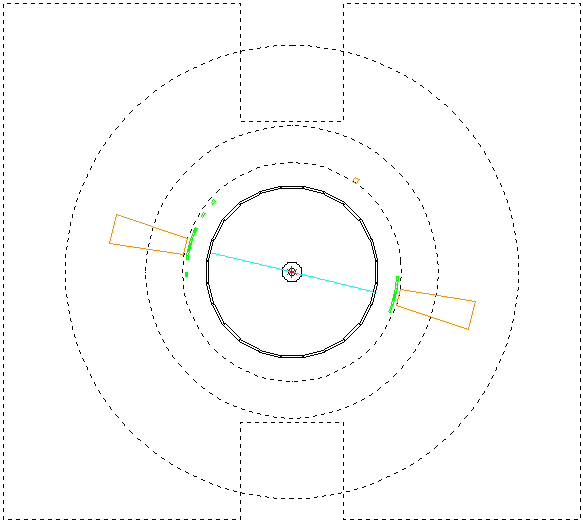
\includegraphics[width=0.49\textwidth]{../figures/grope-ee-w.png}}
	\subfigure[Myonen]{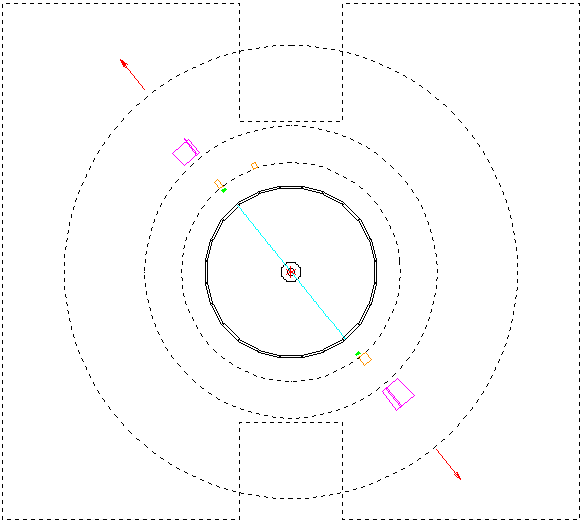
\includegraphics[width=0.49\textwidth]{../figures/grope-mm-w.png}}
	\subfigure[Tauonen]{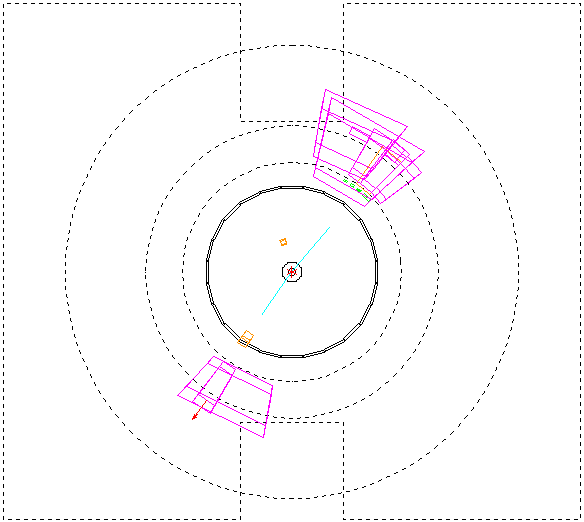
\includegraphics[width=0.49\textwidth]{../figures/grope-tt-w.png}}
	\subfigure[Quarks]{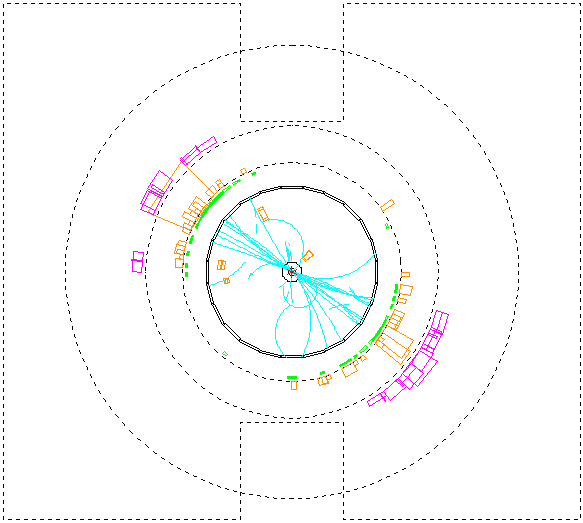
\includegraphics[width=0.49\textwidth]{../figures/grope-qq-w.png}}
	\caption[Detektor-Simulationen für die erwarteten Zerfallsprozesse des Z\textsuperscript0-Bosons]{Detektor-Simulationen für die erwarteten Zerfallsprozesse des Z\textsuperscript0-Bosons. Die Bilder wurden mit GROPE aufgenommen und mit GIMP zur besseren Sichtbarkeit bearbeitet.}
	\label{fig:grope}
\end{figure}
Um später die Separation der Zerfallskanäle durchführen zu können, werden zunächst die einzelnen Zerfallskanäle simuliert und betrachtet. In Abbildung \ref{fig:grope} ist für jeden Zerfallskanal ein Prozess beispielhaft dargestellt.\\

\begin{figure}
	\centering
	\subfigure[$N_\mathrm{charged}$]{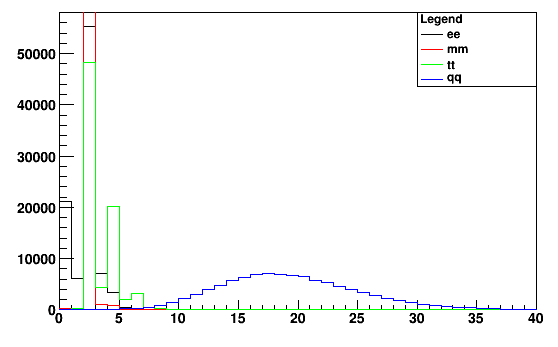
\includegraphics[width=0.49\textwidth]{../figures/Ncharged.png}}
	\subfigure[$P_\mathrm{charged}$]{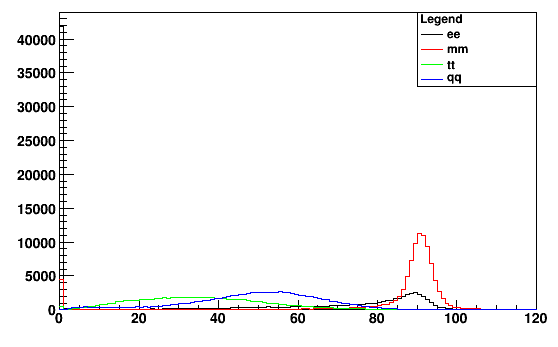
\includegraphics[width=0.49\textwidth]{../figures/Pcharged.png}}
	\subfigure[$E_\mathrm{ecal}$]{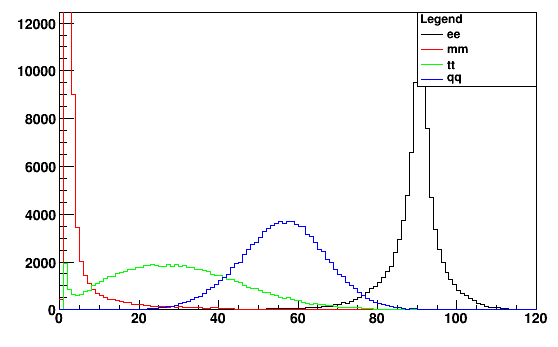
\includegraphics[width=0.49\textwidth]{../figures/E_ecal.png}}
	\subfigure[$E_\mathrm{hcal}$]{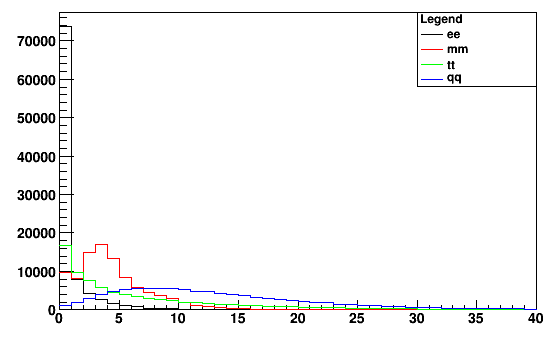
\includegraphics[width=0.49\textwidth]{../figures/E_hcal.png}}
	\subfigure[$\cos\theta$]{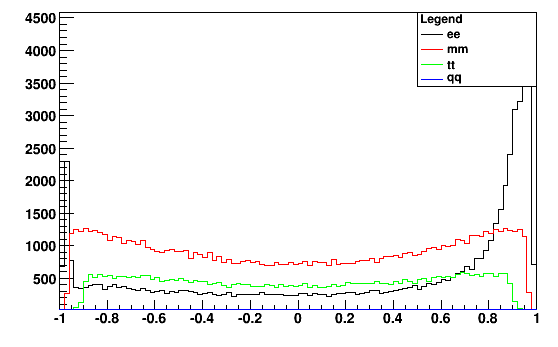
\includegraphics[width=0.49\textwidth]{../figures/cos_thet.png}}
	\caption[Verteilungen der Parameter für die Monte-Carlo-simulierten Daten]{Verteilungen der Parameter für die Monte-Carlo-simulierten Daten.}
	\label{fig:mc}
\end{figure}

Jeder Zerfall lässt sich durch bestimmte Parameter charakterisieren. Dies sind die Anzahl $N_\text{charged}$ der geladenen Spuren im Spurdetektor, $P_\text{charged}$ der Impuls der geladenen Teilchen im Spurdetektor, $E_\text{ecal}$ die an das elektromagnetische Kalorimeter abgegebene Energie, $E_\text{hcal}$ die an das hadronische Kalorimeter abgegebene Energie und $\cos\theta$ der Winkel zwischen einlaufenden und auslaufenden Teilchen. Mit Hilfe der Monte-Carlo-Simulation (siehe Abschnitt \ref{sec:montecarlo}) lassen sich diese Parameter für die einzelnen Zerfallskanäle separat simulieren. Die einzelnen Parameter sind in Abbildung \ref{fig:mc} aufgetragen.\\

Aus diesen Daten lassen sich nun Schnitte festlegen, nach denen die einzelnen Zerfallskanäle aus den experimentell erhaltenen Daten separiert werden können. Zum Festlegen der Schnitte wurde das Skript \code{makeCuts.C} im Anhang \ref{sec:root} entwickelt. Die hierbei vorläufig festgelegten Schnitte sind in Tabelle \ref{tab:cuts} zu finden.\\

\begin{table}
	\centering
	\begin{tabular}{r|p{10 cm}}
		\textbf{Zerfallskanal}&\textbf{Schnitt}\\\hline
		Elektronen&$\left(N_\text{charged}<5 \land E_\text{ecal}\geq74\right) \lor \left(P_\text{charged}=0\land E_\text{ecal}>80\right)$\\
		Myonen&$N_\text{charged}<5 \land E_\text{ecal}<50 \land \left(P_\text{charged}\geq 75 \lor P_\text{charged}<1\right)$\\
		Tauonen&$N_\text{charged}<5 \land E_\text{ecal}<74 \land P_\text{charged}< 75$\\
		Quarks&$N_\text{charged}>7$\\
	\end{tabular}
	\caption{Vorläufig festgelegte Schnitte zur Separation der Zerfallskanäle}
	\label{tab:cuts}
\end{table}

\paragraph{2-Photonen-Prozesse}
Ein in der Simulation nicht berücksichtigter Prozess ist der in \ref{sec:e+e-} beschriebene Prozess der inelastischen Streuung, auch als 2-Photonen-Prozess bezeichnet. Um diese zu eliminieren betrachtet man, wie in Abbildung \ref{fig:2photon} beispielhaft für den elektronischen Zerfallskanal dargestellt, die (normierte) Anzahl an Ereignissen in Abhängigkeit von $P_\text{charged}$ und $E_\text{ecal}$ sowohl der experimentellen als auch der simulierten Daten. Nun sucht man Stellen, an denen in den experimentellen Daten deutlich mehr Ereignisse auftauchen als in den simulierten Daten. Diese sind dann vermutlich auf solche 2-Photonen-Prozesse zurückzuführen und lassen sich durch eine Anpassung der Schnitte eliminieren. Im Rahmen der 2-Photonen-Korrektur wurden die Schnitte der Elektronen und der Tauonen angepasst, in dem jeweils eine zusätzliche Grenze $P_\text{charged}>15$ hinzugefügt wurde.
\begin{figure}
	\centering
	\subfigure[Simulation]{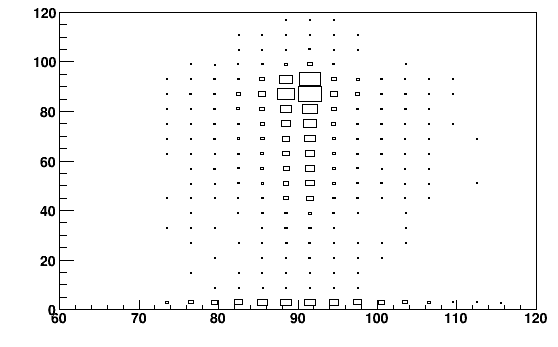
\includegraphics[width=0.49\textwidth]{../figures/ee_2photon_mc.png}}
	\subfigure[Experiment]{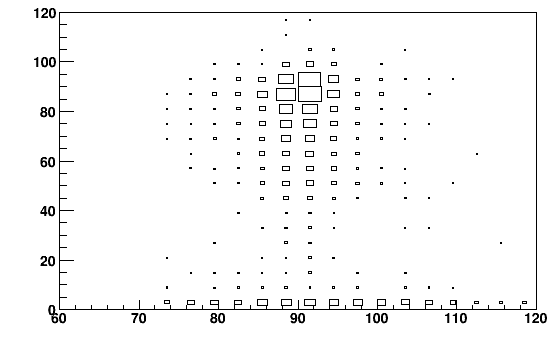
\includegraphics[width=0.49\textwidth]{../figures/ee_2photon_data.png}}
	\caption[Identifizierung der 2-Photon-Ereignisse]{Ereignisse über $P_\text{charged}$ (links) und $E_\text{ecal}$ (unten) zur Identifizierung der 2-Photon-Ereignisse, beispielhaft für Elektronen.}
	\label{fig:2photon}
\end{figure}

\paragraph{Trennung von t-Kanal und s-Kanal}
Wie in Abschnitt \ref{sec:bhabha} beschrieben, existiert für die Elektronen sowohl ein t-Kanal als auch ein s-Kanal, für unseren Versuch ist allerdings nur der s-Kanal relevant. Daher wird die in Abbildung \ref{fig:winkelbhabhatheorie} dargestellte Gleichung \ref{eq:stkanal} an die simulierte $\cos\theta$-Verteilung für Elektronen gefittet und daraus die Parameter $s$ und $t$ bestimmt (siehe Abbildung \ref{fig:stkanal}). Anhand des Fits kann nun eine Obergrenze für $\cos\theta$ festgelegt und der Schnitt entsprechend angepasst werden. Die Obergrenze wurde hier bei $\cos\theta=0.4$ gewählt.

\begin{figure}
	\centering
	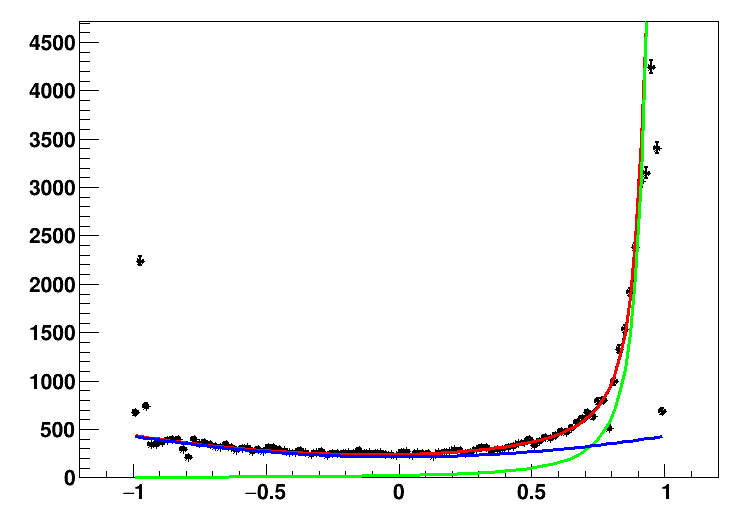
\includegraphics[width=0.8\textwidth]{../figures/stkanal.png}
	\caption[$\cos\theta$-Verteilung für Elektronen mit Fit des erwarteten Verlaufs]{$\cos\theta$-Verteilung für Elektronen mit Fit des erwarteten Verlaufs (rot). Außerdem eingezeichnet sind separat der s-Kanal (blau) und der t-Kanal (grün)}
	\label{fig:stkanal}
\end{figure}

\paragraph{Endgültige Festlegung der Schnitte}
Anhand der Korrekturen durch 2-Photonen-Prozesse und den Einfluss der t-Kanal-Prozesse können nun die Schnitte entsprechend Tabelle \ref{tab:finalcuts} festgelegt werden.

\begin{table}
	\centering
	\begin{tabular}{r|p{11 cm}}
		\textbf{Zerfallskanal}&\textbf{Schnitt}\\\hline
		Elektronen&$\left(\left(N_\text{charged}<5 \land E_\text{ecal}\geq74\right) \lor \left(P_\text{charged}=0\land E_\text{ecal}>80\right)\right)$\newline$\land\cos\theta<0,4\land P_\text{charged}>15$\\
		Myonen&$N_\text{charged}<5 \land E_\text{ecal}<50 \land \left(P_\text{charged}\geq 75 \lor P_\text{charged}<1\right)$\\
		Tauonen&$N_\text{charged}<5 \land E_\text{ecal}<74 \land P_\text{charged}< 75\land P_\text{charged}>15$\\
		Quarks&$N_\text{charged}>7$\\
	\end{tabular}
	\caption{Endgültig festgelegte Schnitte zur Separation der Zerfallskanäle}
	\label{tab:finalcuts}
\end{table}

\subsection{Bestimmung der Partialbreiten}

\subsubsection{Effizienzmatrix}

Die Effizienz $\mathcal{E}_{f_1}^{f_2}$ ist definiert als der Anteil der Fermionen $f_1$, welcher im Schnitt des Fermions $f_2$ vorhanden ist. Die theoretisch optimale Effizienz ist also gegeben durch $\mathcal{E}_{f_1}^{f_2}=\delta_{f_1f_2}$. Die Effizienz berechnet sich aus den simulierten Daten. Für jeden Fermion-Zerfallskanal wird die Anzahl der von den einzelnen Schnitten ausgewählten Ereignisse gezählt und das Verhältnis zur Gesamtanzahl der Ereignisse in diesem Zerfallskanal gebildet: 
\begin{align}
	\mathcal{E}_{f_1}^{f_2}=\frac{N_{f_1}^{f_2}}{N_{f_1}}\text{.}
\end{align}

Die Effizienzen lassen sich nun als Matrix folgendermaßen schreiben:
\begin{align}
	\mathcal{E}&=
	\begin{pmatrix}
		\mathcal{E}_{e}^{e}&
		\mathcal{E}_{\mu}^{e}&
		\mathcal{E}_{\tau}^{e}&
		\mathcal{E}_{q}^{e}\\
		\mathcal{E}_{e}^{\mu}&
		\mathcal{E}_{\mu}^{\mu}&
		\mathcal{E}_{\tau}^{\mu}&
		\mathcal{E}_{q}^{\mu}\\
		\mathcal{E}_{e}^{\tau}&
		\mathcal{E}_{\mu}^{\tau}&
		\mathcal{E}_{\tau}^{\tau}&
		\mathcal{E}_{q}^{\tau}\\
		\mathcal{E}_{e}^{q}&
		\mathcal{E}_{\mu}^{q}&
		\mathcal{E}_{\tau}^{q}&
		\mathcal{E}_{q}^{q}
	\end{pmatrix}
	\\&=
	\begin{pmatrix}
		0,617\pm0,003&0,000011\pm0,000011&0,00106\pm0,00011&0\\
		0,00069\pm0,00009&0,956\pm0,004&0,0111\pm0,0003&0,000020\pm0,000015\\
		0,0055\pm0,0003&0,0427\pm0,0008&0,809\pm0,004&0,00003\pm0,00002\\
		0,00006\pm0,00002&0&0,0068\pm0,0003&0,990\pm0,004
	\end{pmatrix}\text{.}
\end{align}
Der Fehler auf die Effizienzen berechnet sich hierbei mit Hilfe von Gauß'scher Fehlerfortpflanzung aus den Poissonfehlern der Ereignisanzahlen.\\

Die erhaltenen Ereignisse $N_\text{data}$ ergeben sich offensichtlich folgendermaßen mit Hilfe der Effizienzen aus den wahren Werten $N_\text{true}$:
\begin{align}
	\begin{pmatrix}
		N_e^\text{data}\\
		N_\mu^\text{data}\\
		N_\tau^\text{data}\\
		N_q^\text{data}\\
	\end{pmatrix}
	&=
	\mathcal{E}\cdot
	\begin{pmatrix}
	N_e^\text{true}\\
	N_\mu^\text{true}\\
	N_\tau^\text{true}\\
	N_q^\text{true}\\
	\end{pmatrix}\text{.}
\end{align}

Die wahre Anzahl der Ereignisse berechnet sich also mit Hilfe der inversen Matrix $\mathcal{E}^{-1}$ folgendermaßen:
\begin{align}
\begin{pmatrix}
N_e^\text{true}\\
N_\mu^\text{true}\\
N_\tau^\text{true}\\
N_q^\text{true}\\
\end{pmatrix}
&=
\mathcal{E}^{-1}\cdot
\begin{pmatrix}
N_e^\text{data}\\
N_\mu^\text{data}\\
N_\tau^\text{data}\\
N_q^\text{data}\\
\end{pmatrix}\text{.}
\end{align}

Zur Invertierung der Matrix wird das Script \code{useMatrix.C} in Anhang \ref{sec:root} verwendet. Zur Berechnung der Fehler der Elemente der inversen Matrix, wird die ursprüngliche Matrix mit Hilfe einer Gaußverteilung mit der Standardabweichung $s_\mathcal{E}$ verrauscht und invertiert. Nun werden die Standardabweichungen der resultierenden Verteilungen als Fehler für die Matrixelemente angegeben.

\subsubsection{Wirkungsquerschnitte}

Nachdem nun aus den aus den Daten erhaltenen Anzahlen die wahren Anzahlen berechnet wurden, werden mit Hilfe der im Versuch angegebenen Luminositäten $L$ die Wirkungsquerschnitte ausgerechnet und mit Hilfe der Strahlungskorrekturwerte $c$ korrigiert \cite{anleitungalt}:
\begin{align}
	\sigma_f&=\frac{N_f^\text{true}}{L}+c\text{.}
\end{align}

Die hierbei erhaltenen Wirkungsquerschnitte werden nun in Abhängigkeit der Schwerpunktsenergien in Abbildung \ref{fig:wirkungsquerschnitte} dargestellt. Mit Hilfe von Gleichung \ref{eq:partialbreiten} aus Abschnitt \ref{sec:partialbreiten} wurde der erwartete Verlauf des Wirkungsquerschnittes an die Schaubilder gefittet, um die $Z^0$-Masse $M_Z$ und die Partialbreiten $\Gamma_e$, $\Gamma_\mu$, $\Gamma_\tau$ sowie $\Gamma_q$ zu ermitteln.\\

\begin{figure}
	\centering
	\subfigure[Elektronen]{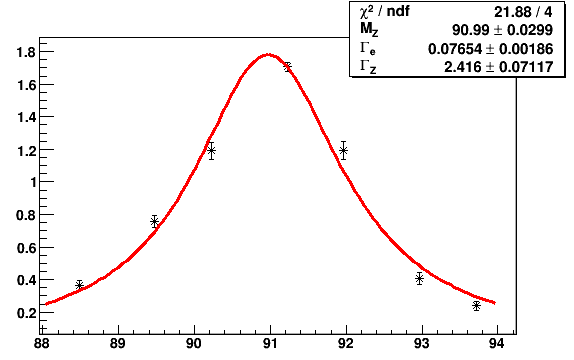
\includegraphics[width=0.49\textwidth]{../figures/elektronen.png}}
	\subfigure[Myonen]{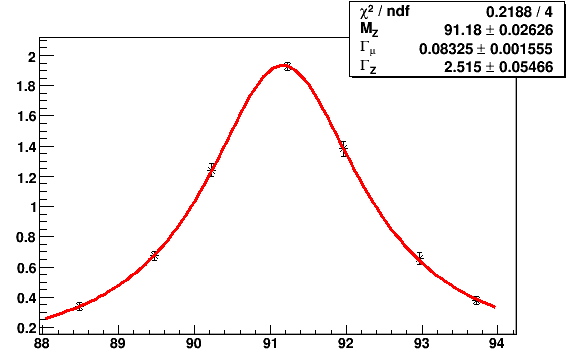
\includegraphics[width=0.49\textwidth]{../figures/myonen.png}}
	\subfigure[Tauonen]{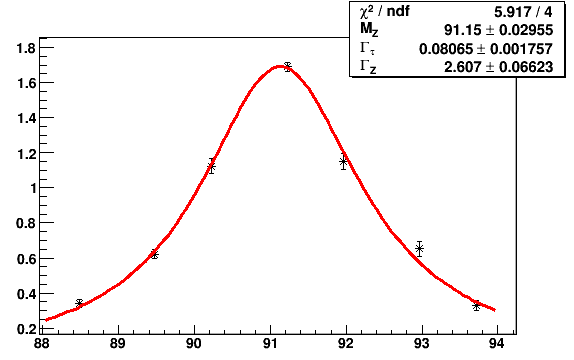
\includegraphics[width=0.49\textwidth]{../figures/tauonen.png}}
	\subfigure[Quarks]{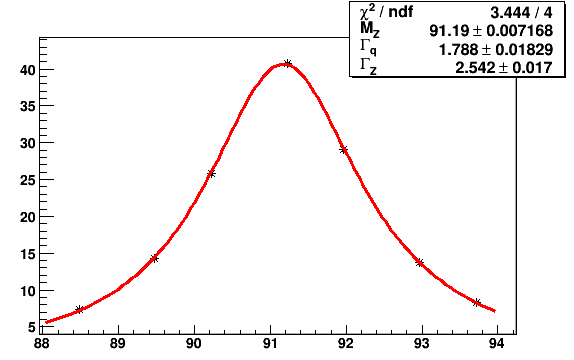
\includegraphics[width=0.49\textwidth]{../figures/quarks.png}}
	\subfigure[Leptonen]{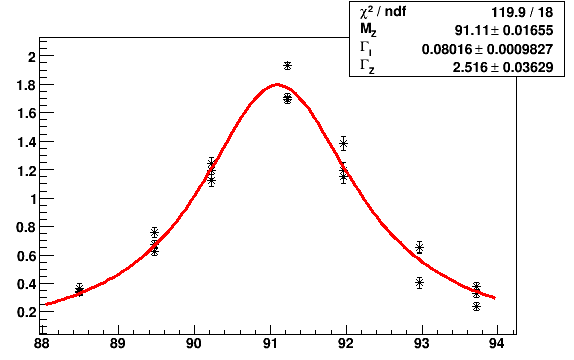
\includegraphics[width=0.49\textwidth]{../figures/leptonen.png}\label{fig:wirkungsquerschnitte:leptonen}}
	\subfigure[Leptonen (gewichtet)]{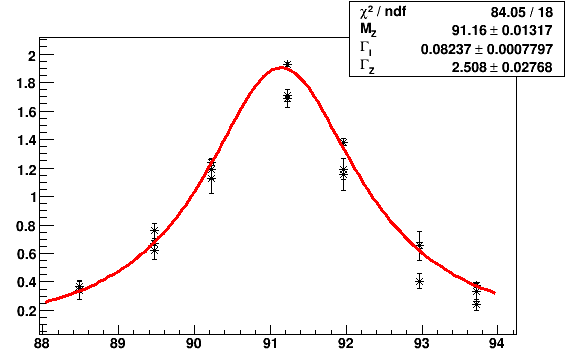
\includegraphics[width=0.49\textwidth]{../figures/leptonen_gewichtet.png}\label{fig:wirkungsquerschnitte:leptonengewichtet}}
	\caption[Wirkungsquerschnitte in Abhängigkeit der Schwerpunktsenergien]{Wirkungsquerschnitte in Abhängigkeit der Schwerpunktsenergien mit Fits zur Ermittelung der Z\textsuperscript0-Masse und der Partialbreiten.}
	\label{fig:wirkungsquerschnitte}
\end{figure}

Außerdem wurde unter der Annahme von Leptonenuniversalität (siehe Gleichung \ref{eq:leptonenuniversalitaet} in Abschnitt \ref{sec:partialbreiten}) in Abbildung \ref{fig:wirkungsquerschnitte:leptonen} die Partialbreite $\Gamma_{e/\mu/\tau}$ der Leptonen mit Hilfe der Daten aller leptonischen Zerfallskanäle bestimmt. Um die Qualität des Fits zu verbessern wurde eine Wichtung nach den $\frac{\chi^2}{\mathrm{ndf}}$-Werten der einzelnen Zerfallskanäle durchgeführt. Dies wurde solange wiederholt, bis der $\frac{\chi^2}{\mathrm{ndf}}$-Wert des gesamten Fits nicht mehr besser wurde. Das Ergebnis dieses gewichteten Fits ist in Abbildung \ref{fig:wirkungsquerschnitte:leptonengewichtet} dargestellt.

\subsubsection{Ergebnisse}

Als Ergebnis für die Gesamtzerfallsbreite $\Gamma_Z$ und die Masse $M_Z$ des $Z^0$-Bosons werden die Ergebnisse für den gewichteten Leptonenfit sowie für den Quarkfit gemittelt. Dabei erhalten wir folgende Ergebnisse:
\begin{alignat}{3}
	&M_Z^\text{Quarks}&&=&\,(91,190\pm0,007)\,\si{GeV}\text{,}\\
	&M_Z^\text{Leptonen}&&=&\,(91,160\pm0,013)\,\si{GeV}\text{,}\\
	&\Gamma_Z^\text{Quarks}&&=&(2542\pm17)\,\si{MeV}\text{,}\\
	&\Gamma_Z^\text{Leptonen}&&=&(2510\pm30)\,\si{MeV}\text{,}\\
	&M_Z&&=&\,(91,183\pm0,006)\,\si{GeV}\text{,}\\
	&\Gamma_Z&&=&(2534\pm15)\,\si{MeV}\text{.}
\end{alignat}

Für die leptonische Zerfallsbreite werden die Ergebnisse aus dem gewichteten leptonischen Fit verwendet. Für die leptonische und hadronische Zerfallsbreite ergeben sich folgende Ergebnisse:
\begin{alignat}{3}
	&\Gamma_{e/\mu/\tau}&&=&(82,4\pm0,8)\,\si{MeV}\text{,}\\
	&\Gamma_l&&=3\cdot\Gamma_{e/\mu/\tau}=\,\,&(247\pm2)\,\si{MeV}\text{,}\\
	&\Gamma_q&&=&(1788\pm18)\,\si{MeV}\text{.}
\end{alignat}

Für die Verzweigungsverhältnisse $\mathrm{BR}_l$ und $\mathrm{BR}_q$ mit
\begin{align}
	\mathrm{BR}_f&=\frac{\Gamma_f}{\Gamma_Z}
\end{align}
erhalten wir folgende Ergebnisse:
\begin{alignat}{3}
	&\mathrm{BR}_l&&=&\,(9,74\pm0,10)\,\%\text{,}\\
	&\mathrm{BR}_q&&=&(70,6\pm0,8)\,\%\text{.}
\end{alignat}

\subsection{Bestimmung der Anzahl der Neutrinogenerationen}

Aus der Differenz zwischen der gesamten Zerfallsbreite $\Gamma_Z$ und der Summe der leptonischen und hadronischen Zerfallsbreiten $\Gamma_l+\Gamma_q$ lässt sich nun die unsichtbare Zerfallsbreite des Neutrino-Zerfallskanals bestimmen:
\begin{align}
	\Gamma_\nu&=\Gamma_Z-\left(\Gamma_l+\Gamma_q\right)=(500\pm20)\,\si{MeV}\text{.}
\end{align}

Aus Gleichung \ref{eq:neutrinos} in Abschnitt \ref{sec:partialbreiten} erhalten wir die Zerfallsbreite $\Gamma_{\nu_e/\nu_\mu/\nu_\tau}$ für eine einzelne Neutrinogeneration und berechnen damit aus der unsichtbaren Zerfallsbreite die Anzahl der Neutrinogenerationen:
\begin{align}
	N_\nu&=\frac{\Gamma_\nu}{\Gamma_{\nu_e/\nu_\mu/\nu_\tau}}=3,01\pm0,14\text{.}
\end{align}

\subsection{Bestimmung des Weinbergwinkels}

Zur Berechnung des Weinbergwinkels aus den gegebenen Daten des OPAL-Experiments verwenden wir die in Abschnitt \ref{sec:asymm} diskutierte Vorwärts-Rückwärts-Asymmetrie. Wir nutzen hierfür die Daten des myonischen Zerfallskanals. Zur Berechnung der Asymmetrie bestimmen wir aus den Messdaten die Summe aller Vorwärts-Ereignisse $\Sigma_\text{Vorwärts}=\cos\theta>0$ und die Summe aller Rückwärts-Ereignisse $\Sigma_\text{Rückwärts}=\cos\theta<0$ und berechnen die Asymmetrie folgendermaßen (vgl. Gleichung \ref{eq:asymm}):
\begin{align}
	A_\text{FB}&=\frac{\Sigma_\text{Vorwärts}-\Sigma_\text{Rückwärts}}{\Sigma_\text{Vorwärts}+\Sigma_\text{Rückwärts}}=0,077\pm0,018\text{.}
\end{align}

Daraus bestimmen wir mit Hilfe von Gleichung \ref{eq:weinberg} $\sin^2\theta_W$ folgendermaßen:
\begin{align}
	\sin^2\theta_W&=\frac14\left(1-\sqrt{\frac{A_{FB}}3}\right)=0,21\pm0,02\text{.}
\end{align}
Der Fehler berechnet sich hierbei mit Hilfe von Gauß'scher Fehlerfortpflanzung aus dem Poissonfehler auf die Ereignisanzahl.